%----------------------------------------------------------------------------------------
%	PACKAGES & THEMES
%----------------------------------------------------------------------------------------

\documentclass[8pt]{beamer}

\usepackage{etex}
\mode<presentation> {

\usetheme{Vilanova}
}



\usepackage[english]{babel}
\usepackage[utf8]{inputenc}
\usepackage{array}
\usepackage{chronology}
\let\CHRONOLOGY\chronology
\let\endCHRONOLOGY\endchronology
\def\chronology{\shorthandoff{;}\CHRONOLOGY}
\def\endchronology{\endCHRONOLOGY\shorthandon{;}}
\usepackage{pstricks}
\usepackage{graphicx}
\usepackage{booktabs}
\usepackage{amsmath,amssymb,amsthm}
\usepackage{xcolor}
\usepackage{textpos}
\usepackage{tikz}
\usepackage{xmpincl}
\usetikzlibrary{arrows}
\usepackage{pifont}

\usepackage{listings,color}

\definecolor{listcomment}{rgb}{0.0,0.5,0.0}
\definecolor{listkeyword}{rgb}{0.0,0.0,0.5}
\definecolor{listnumbers}{gray}{0.65}
\definecolor{listlightgray}{gray}{0.955}
\definecolor{listwhite}{gray}{1.0}


%% \setbeamertemplate{background canvas}{\includegraphics
%%    [width=\paperwidth,height=\paperheight]{./images/title.pdf}}

\AtBeginSection[]
{
\addtocounter{framenumber}{-1}
\begin{frame}
\frametitle{Sommaire}
\tableofcontents[currentsection]
\end{frame}}

%----------------------------------------------------------------------------------------
%	PAGE TITRE
%----------------------------------------------------------------------------------------
\title{ Insight on the applications framework}
\includexmp{images/cc}
\subtitle{OTB functions without templates}
\author{OTB development team}% date and event here
\date{3 - 5 june 2015, Toulouse}

\pgfdeclareimage[height=96mm,width=128mm]{background}{images/fondsClairSansLogo}
\pgfdeclareimage[height=0.2cm]{cc}{images/CC-licence.png}
\setbeamertemplate{background}{\pgfuseimage{background}}
\pgfdeclareimage[height=0.6cm]{logoIncrust}{images/logoIncrust}
\logo{
\begin{tabular}{p{0.22\textwidth}p{0.58\textwidth}p{0.1\textwidth}p{0.1\textwidth}}
\href{http://creativecommons.org/licenses/by-sa/3.0/}{\pgfuseimage{cc}}
& \vspace{-0.03\textwidth} \scriptsize{} % date and event here
&  & \href{http://www.orfeo-toolbox.org}{\pgfuseimage{logoIncrust}}\\
\end{tabular}
}


\begin{document}
\begin{frame}
\titlepage
\end{frame}

\section{OTB applications in a nutshell}

\begin{frame}
\frametitle{Applications: code once, use (nearly) everywhere}
\begin{columns}
\column{0.5\textwidth}
\begin{itemize}
\item 81 applications shipped with OTB
\item 1 application $=$ 1 dynamic library (plugin) (otbapp\_*.so)
\item Auto generation, auto-doc
\item Application C++ API not specific to OTB
\item Wrappers build upon Application engine
\begin{itemize}
\item Command Line
\item Qt (used in Monteverdi2 and QGIS (custom version of otb app))
\item Python (with SWIG) other languages are wrapped (Java,Lua,PyQt) 
\end{itemize}
\item Easy integration in external system 
\end{itemize}
\column{0.5\textwidth}
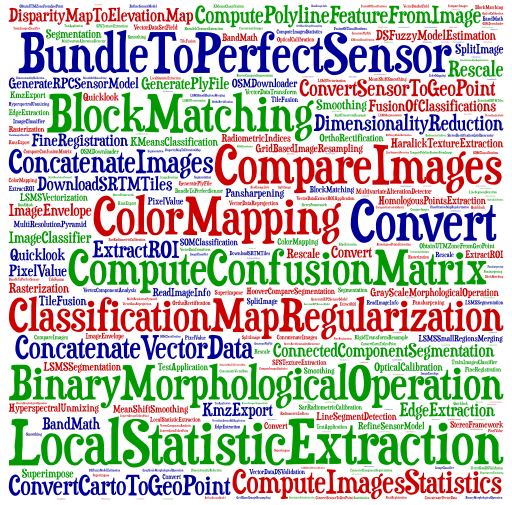
\includegraphics[width=\textwidth]{images/cloud_applications}
\end{columns}
\end{frame}



\begin{frame}[fragile]
%\frametitle{Applications: CLI}
\begin{scriptsize}
\vspace{-0.5cm}\begin{verbatim}
$ otbcli_OrthoRectification

This is the OrthoRectification application, version 5.0.0
This application allows to ortho-rectify optical images from supported sensors.

Complete documentation: http://www.orfeo-toolbox.org/Applications/OrthoRectification.html

Parameters: 
-progress                <boolean>        Report progress 
MISSING -io.in                   <string>         Input Image  (mandatory)
MISSING -io.out                  <string> [pixel] Output Image  [pixel=uint8/uint16/int16/uint32/int32/float/double] (default value is float) (mandatory)
-map                     <string>         Output Cartographic Map Projection [utm/lambert2/lambert93/wgs/epsg] (mandatory, default value is utm)
-map.utm.zone            <int32>          Zone number  (mandatory, default value is 31)
-map.utm.northhem        <boolean>        Northern Hemisphere  (optional, off by default)
-map.epsg.code           <int32>          EPSG Code  (mandatory, default value is 4326)
-outputs.mode            <string>         Parameters estimation modes [auto/autosize/autospacing/outputroi/orthofit] (mandatory, default value is auto)
MISSING -outputs.ulx             <float>          Upper Left X  (mandatory)
MISSING -outputs.uly             <float>          Upper Left Y  (mandatory)
MISSING -outputs.sizex           <int32>          Size X  (mandatory)
MISSING -outputs.sizey           <int32>          Size Y  (mandatory)
MISSING -outputs.spacingx        <float>          Pixel Size X  (mandatory)
MISSING -outputs.spacingy        <float>          Pixel Size Y  (mandatory)
-outputs.lrx             <float>          Lower right X  (optional, off by default)
-outputs.lry             <float>          Lower right Y  (optional, off by default)
-outputs.ortho           <string>         Model ortho-image  (optional, off by default)
-outputs.isotropic       <boolean>        Force isotropic spacing by default  (optional, on by default)
-outputs.default         <float>          Default pixel value  (optional, on by default, default value is 0)
-elev.dem                <string>         DEM directory  (optional, off by default)
-elev.geoid              <string>         Geoid File  (optional, off by default)
-elev.default            <float>          Default elevation  (mandatory, default value is 0)
-interpolator            <string>         Interpolation [bco/nn/linear] (mandatory, default value is bco)
-interpolator.bco.radius <int32>          Radius for bicubic interpolation  (mandatory, default value is 2)
-opt.rpc                 <int32>          RPC modeling (points per axis)  (optional, off by default, default value is 10)
-opt.ram                 <int32>          Available RAM (Mb)  (optional, off by default, default value is 128)
-opt.gridspacing         <float>          Resampling grid spacing  (optional, on by default, default value is 4)
-inxml                   <string>         Load otb application from xml file  (optional, off by default)

Examples: 
otbcli_OrthoRectification -io.in QB_TOULOUSE_MUL_Extract_500_500.tif -io.out QB_Toulouse_ortho.tif
\end{verbatim}
\end{scriptsize}
\end{frame}

\begin{frame}[fragile]
\frametitle{Applications: Qt graphical interface (parameters)}
\begin{center}
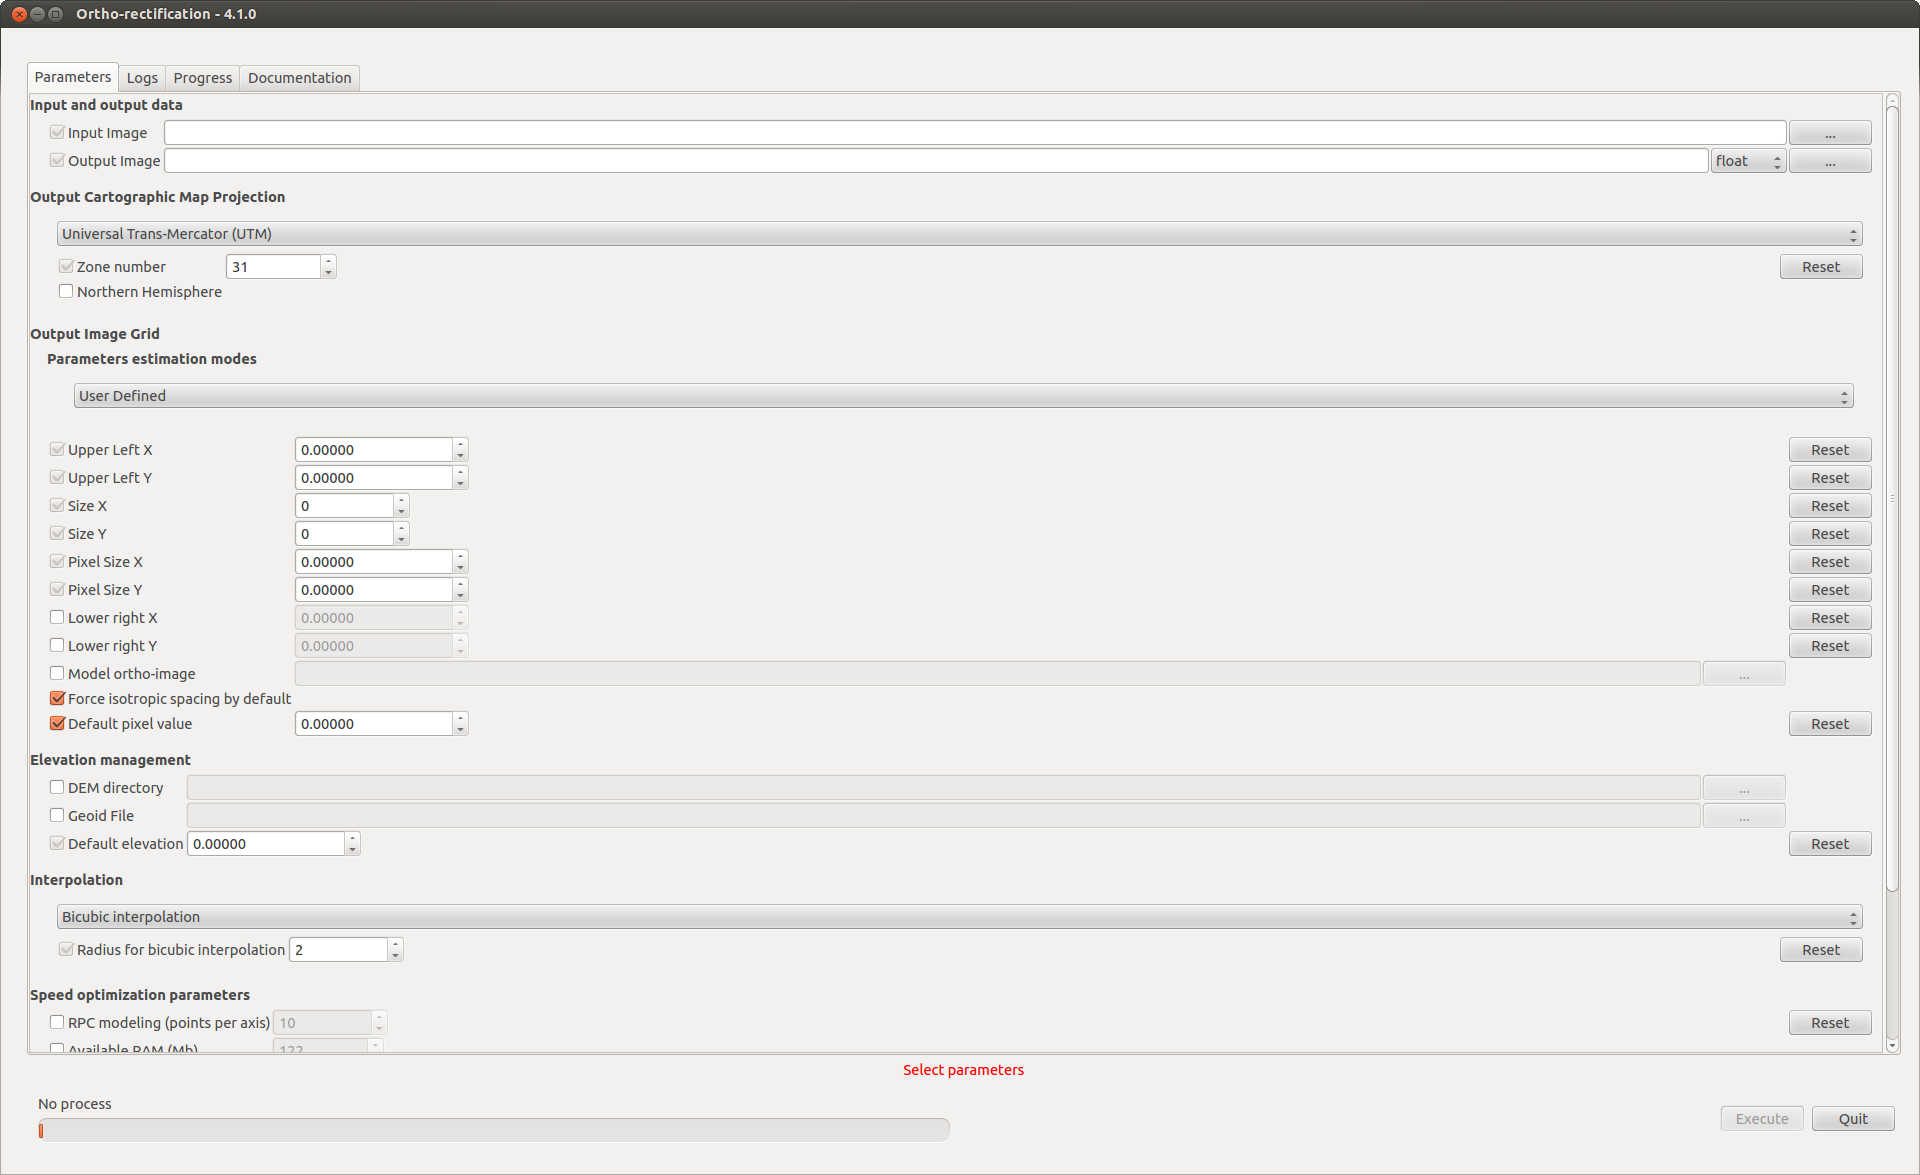
\includegraphics[width=0.9\textwidth]{images/app_parameters.png}
\end{center}
\end{frame}


\begin{frame}[fragile]
\frametitle{Applications: Qt graphical interface (documentation)}
\begin{center}
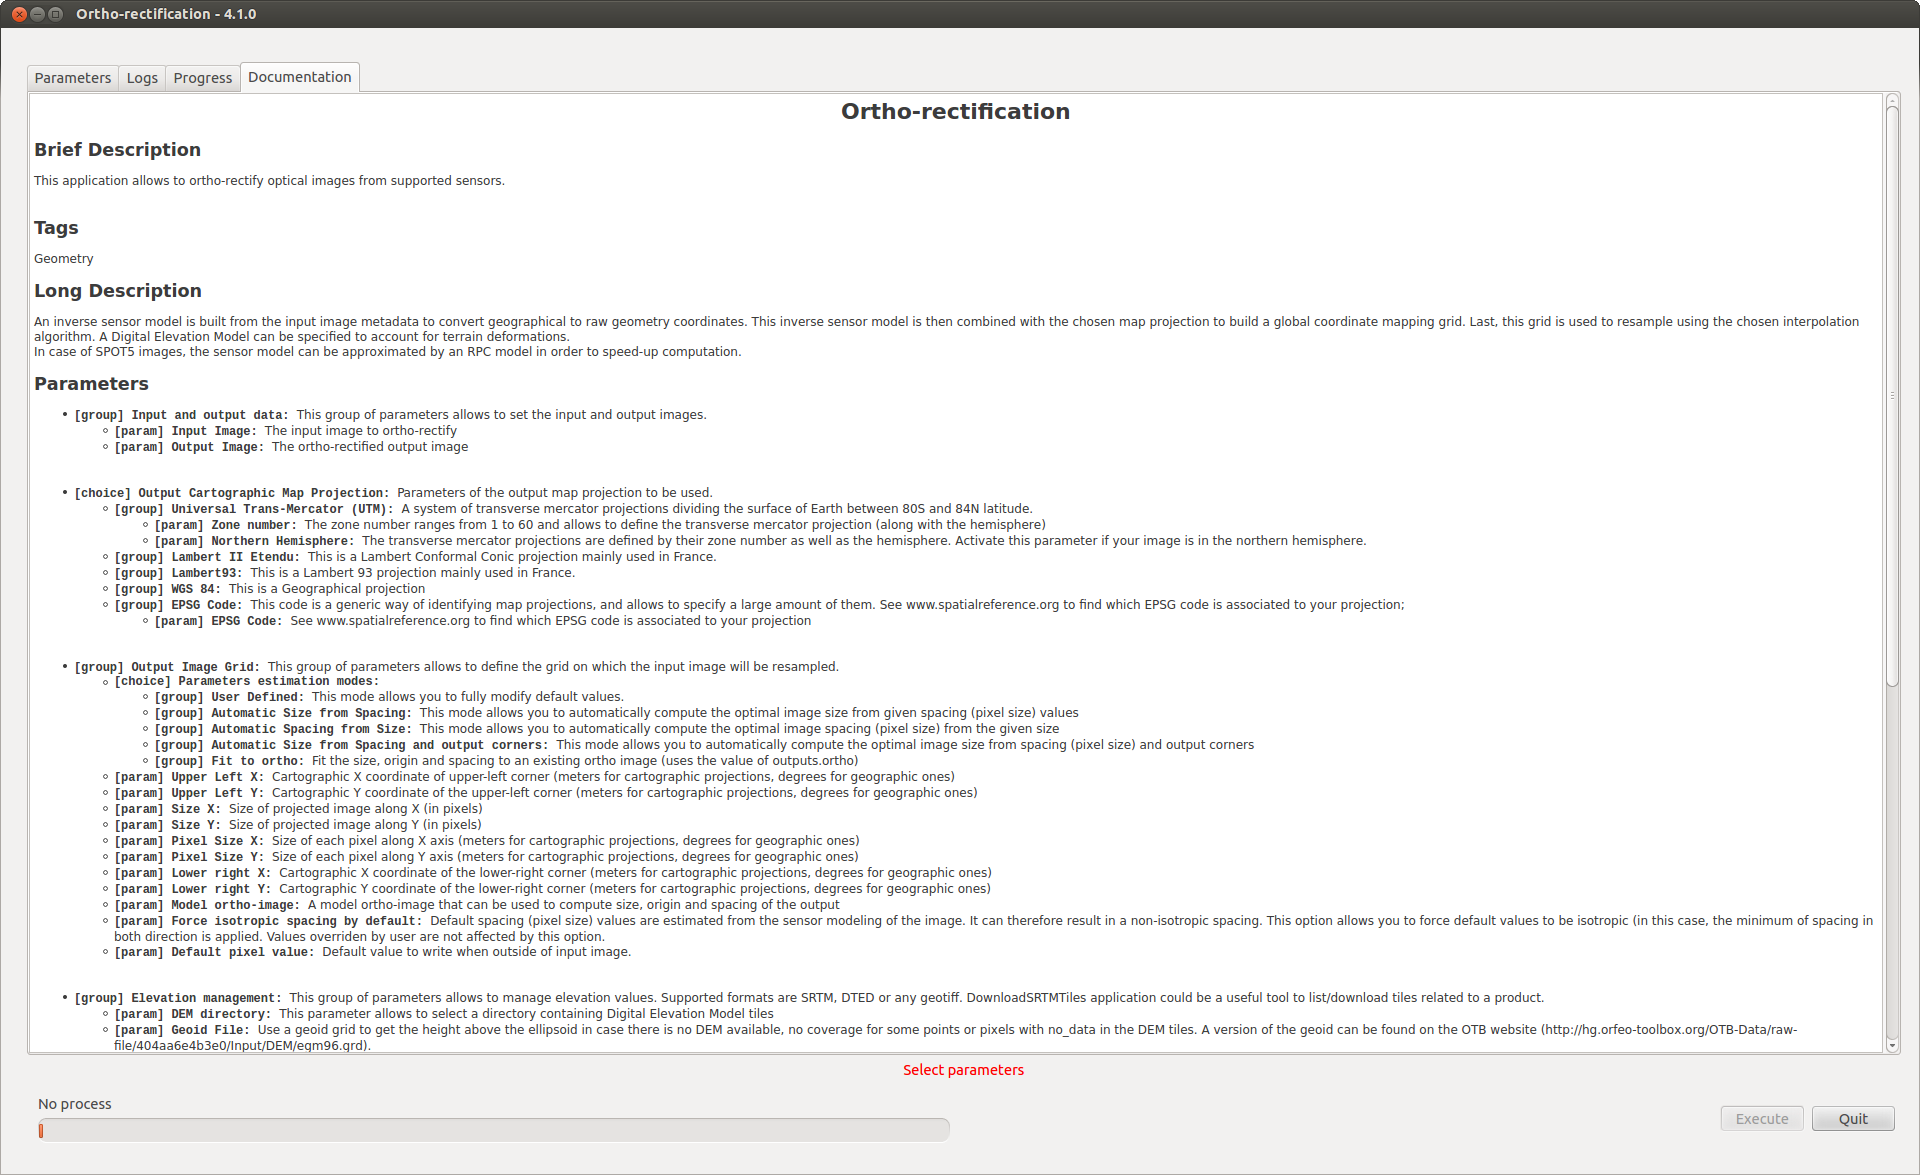
\includegraphics[width=0.9\textwidth]{images/app_doc.png}
\end{center}
\end{frame}

\begin{frame}[fragile]
\frametitle{OTB in QGIS}
\begin{center}
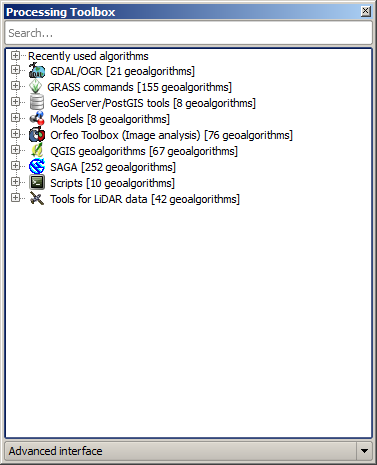
\includegraphics[width=0.4\textwidth]{images/otb_qgis.png}
\end{center}
\end{frame}

\begin{frame}[fragile]
\frametitle{Applications: Python interface}
\begin{lstlisting}[language=python,breaklines=true,breakatwhitespace=true,frame = tb,framerule = 0.25pt,fontadjust,backgroundcolor={\color{listlightgray}},basicstyle = {\ttfamily\tiny},keywordstyle = {\ttfamily\color{listkeyword}\textbf},identifierstyle = {\ttfamily},commentstyle = {\ttfamily\color{listcomment}\textit},stringstyle = {\ttfamily},showstringspaces = false,showtabs = false,numbers = none,numbersep = 6pt, numberstyle={\ttfamily\color{listnumbers}},tabsize = 2]
#!/usr/bin/python 

# Import the otb applications package 
import otbApplication 

# The following line creates an instance of the OrthoRectification application 
OrthoRectification = otbApplication.Registry.CreateApplication("OrthoRectification") 

# The following lines set all the application parameters: 
OrthoRectification.SetParameterString("io.in", "QB_TOULOUSE_MUL_Extract_500_500.tif") 

OrthoRectification.SetParameterString("io.out", "QB_Toulouse_ortho.tif") 

# The following line execute the application 
OrthoRectification.ExecuteAndWriteOutput()
\end{lstlisting}
\end{frame}

\section{Inside OTB applications}

\begin{frame}
\frametitle{Application engine}
\begin{itemize}
\item C++ library inside the OTB library
\item Wrappers for parameters definition (numerical, groups of parameters,
choice parameter) and also
parameters related to OTB types (images, vector, image list)
\item Application definition  
\begin{itemize}
\item Application name, documentation\ldots
\item   /* Implement this method to add parameters */ virtual void DoInit() = 0;
\item /* Implement this method to update non valued parameters */ virtual void DoUpdateParameters() = 0;
\item /* Implement this method to build the output */ virtual void DoExecute() = 0;
\end{itemize}
\item Goodies
\begin{itemize}
\item Handle dependencies between parameters
\item Logger (warniong, error, progress\ldots)
\item Tags
\item Auto doc generation
\item Serialization (XML files) 
-outxml - Save otb application to xml file: Save otb application to xml file
-inxml  - Load otb application from xml file  (optional, off by default)
\end{itemize}
\end{itemize}
\end{frame}

\begin{frame}[fragile]
\frametitle{Applications: Python interface}
\begin{lstlisting}[language=xml,breaklines=true,breakatwhitespace=true,frame = tb,framerule = 0.25pt,fontadjust,backgroundcolor={\color{listlightgray}},basicstyle = {\ttfamily\tiny},keywordstyle = {\ttfamily\color{listkeyword}\textbf},identifierstyle = {\ttfamily},commentstyle = {\ttfamily\color{listcomment}\textit},stringstyle = {\ttfamily},showstringspaces = false,showtabs = false,numbers = none,numbersep = 6pt, numberstyle={\ttfamily\color{listnumbers}},tabsize = 2]
<?xml version="1.0" ?>
<OTB>
    <version>3.18</version>
    <build>18-05-2013</build>
    <platform>Linux</platform>
    <application>
        <name>Smoothing</name>
        <descr>Apply a smoothing filter to an image</descr>
        <doc>
            <name>Smoothing</name>
            <longdescr>This application applies smoothing filter to an image. Either gaussian, mean, or anisotropic diffusion are available.</longdescr>
            <authors>OTB-Team</authors>
            <limitations>None</limitations>
            <seealso> </seealso>
            <tags>
                <tag>Image Filtering</tag>
            </tags>
        </doc>
        <parameter mandatory="true">
            <key>in</key>
            <type>InputImage</type>
            <name>Input Image</name>
            <value>/home/rashad/repos/orfeo/OTB-Data/Input/poupees.tif</value>
        </parameter>
        <parameter mandatory="true">
            <key>out</key>
            <type>OutputImage</type>
            <name>Output Image</name>
            <value>/home/rashad/repos/orfeo/build/OTB_/test-build/Testing/Temporary/apTvUtSmoothingTest_OutXML.tif</value>
        </parameter>
        <parameter mandatory="true">
            <key>type</key>
            <type>Choice</type>
            <name>Smoothing Type</name>
            <value>mean</value>
        </parameter>
    </application>
</OTB>
\end{lstlisting}
\end{frame}


\begin{frame}
\frametitle{Application wrapper}
The general philosophy of this new framework is to have to write the processing
only once, and then use it from whatever environment, programming language or
software you want through one of these access points.

\begin{block}{CLI}
\begin{itemize}
\item itk Object
\item Pointer to an application (load the application)
\item Parse the command line and pilot application
\item Way that we access OTB processing in graphical environnement (mvd2, qgis\ldots)
\end{itemize}
\end{block}

\begin{block}{Qt}
\begin{itemize}
\item QApplication
\item Wrap application parameters types in Qt objects
\end{itemize}
\end{block}

\begin{block}{SWIG}
\begin{itemize}
\item Wrap ApplicationEngine classes with SWIG
\end{itemize}
\end{block}
\end{frame}

\begin{frame}
\frametitle{Applications framework is}
\begin{itemize}
\item Standard way to distribute processing chain based on OTB
\item Showcase for OTB features
\end{itemize}
\end{frame}

\begin{frame}
\frametitle{Applications framework is not (yet)}
\begin{itemize}
\item Wrapper of all OTB classes ($\neq$ WrapITK)
\item An external project based on the library (like ice or MVD). OTB
Applications are included in the library source as a set of modules in
version 5.0.
\item Scheduler of OTB process (applications read and write on disk)
\end{itemize}
\end{frame}

\section{Discussion for future of OTB applications}

\begin{frame}
\frametitle{What-s new for applications in OTB 5.0}
\begin{itemize}
\item Not much\ldots
\item Applications are now stored in a group of modules
\item 24 modules (change detection, mathParser, Segmentation, Fusion\ldots)
\item Currently 81 applications
\end{itemize}
\end{frame}

\begin{frame}
\frametitle{Discussion for future of OTB applications}
\begin{itemize}
\item New applications in the OTB ? Ideas?  
\item Improve integration of OTB-Applications in external projects?
\item Improve documentation (internationalization\ldots)
\end{itemize}
\end{frame}

\end{document}
